\section{音声信号処理}
音声にはフォルマントや基本周波数(ピッチ)など,様々な周波数的な特徴が存在している.フォルマントは母音や子音を知覚するため,ピッチはアクセントやイントネーションを表現するために重要なものである.このような音声信号の持つ複雑さから,時間波形のままその特徴を分析することは困難である.これに対し,本節では音声の特徴を捉えやすくするための信号処理について説明する.

\subsection{音声のフーリエ変換}
音声の時間波形から周波数領域の情報を得るためには、フーリエ変換(Fourier transform)が用いられる。音声は通常マイクロフォンで収録され、コンピュータ内で処理される際には、アナログ信号ではなくデジタル信号として扱われる。このデジタル信号は、サンプリング周波数と量子化ビット数に従って離散化されている。離散化された信号に対しては、離散フーリエ変換(discrete Fourier transform; DFT)が適用される。また,信号の系列長をゼロパディングして2のべき乗の長さに調整すれば,計算量を抑えた高速フーリエ変換(fast Fourier transform; FFT)を用いることができる.

離散信号を$x\lrsq{\numLower}$,それに対するフーリエ変換を$X\lrsq{\freqLower}$とする.ここで,$\numLower$はサンプルのインデックス,$\freqLower$は周波数インデックスである.$X\lrsq{\freqLower}$は複素数であるから,以下のように極座標表示することができる.
\begin{align}
    X\lrsq{\freqLower} & = \Re\lr{X\lrsq{\freqLower}} + \imUnit\Im\lr{X\lrsq{\freqLower}}    \\
                       & = \lrAbs{X\lrsq{\freqLower}}\exp^{\imUnit\angle X\lrsq{\freqLower}}
\end{align}
ここで,$\lrAbs{X\lrsq{\freqLower}}$は振幅特性(振幅スペクトル),$\angle X\lrsq{\freqLower}$は位相特性(位相スペクトル)であり,
\begin{gather}
    \lrAbs{X\lrsq{\freqLower}} = \sqrt{\Re\lr{X\lrsq{\freqLower}}^{2} + \Im\lr{X\lrsq{\freqLower}}^{2}} \\
    \angle X\lrsq{\freqLower} = \tan^{-1} \frac{\Im\lr{X\lrsq{\freqLower}}}{\Re\lr{X\lrsq{\freqLower}}}
\end{gather}
と表される.また,$\lrAbs{X\lrsq{\freqLower}}^2$はパワースペクトルと呼ばれる.これにより,信号中にどのような周波数成分がどれくらい含まれているかを調べることができる.しかし,音声はフォルマントやピッチが時々刻々と変化するため,信号全体に対して直接フーリエ変換を適用したとしても有用な結果が得られない.このような音声の持つ非定常性の問題に対して,十分短い時間幅においては信号の定常性が成り立つという仮定のもと,短時間フーリエ変換(short-time Fourier transform; STFT)が用いられる.STFTでは,音声信号に対して窓関数による窓処理を適用し,短時間に区切られた信号それぞれに対してDFTを適用する.ここで,窓処理とはある特定の窓関数と音声信号を時間領域でかけ合わせることであり,窓関数の時間幅を窓長という.また,窓関数を時間方向にシフトするときの時間幅をシフト幅という.STFTには,時間分解能と周波数分解能の間にトレード・オフの関係がある.窓長が長い場合には周波数分解能が向上する一方,時間分解能が低下する.窓長が短い場合にはその逆となる.音声信号$x\lrsq{\numLower}$のSTFTを時刻$\timeLower$,周波数インデックスを$\freqLower$として$X\lrsq{\timeLower, \freqLower}$と表すと,$X\lrsq{\timeLower, \freqLower}$は時間周波数領域における複素数となる.これを複素スペクトログラムと呼ぶ.また,$|X\lrsq{\timeLower, \freqLower}|$を振幅スペクトログラム,$\angle X\lrsq{\timeLower, \freqLower}$を位相スペクトログラム,
$\lrAbs{X\lrsq{\timeLower, \freqLower}}^{2}$をパワースペクトログラムと呼ぶ.「小さな鰻屋に,熱気のようなものがみなぎる」と発話した音声に対し,窓関数としてハニング窓を用いた上で,複数の窓長・シフト幅によって計算した対数パワースペクトログラムを,図~\ref{sec2:fig:log_power_spectrograms}に示す.窓長が\SI{100}{\ms}と長い場合には周波数分解能が高いが,時間分解能が低下することでスペクトルの時間変化が滑らかでないことがわかる.一方,窓長が\SI{12.5}{\ms}と短い場合には時間分解能が高いが,周波数分解能が低下することでスペクトルがぼやけていることがわかる.これが窓長に対する時間分解能と周波数分解能のトレード・オフであり,窓長\SI{25}{\ms}や\SI{50}{ms}が程よいパラメータであることがわかる.
\begin{figure}[tb]
    \centering
    \begin{subfigure}[b]{0.48\textwidth}
        \centering
        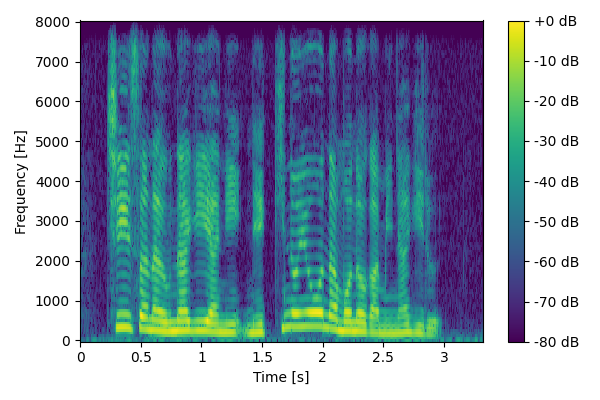
\includegraphics[width=\textwidth]{./figure/sec2/spectrogram_1.png}
        \caption{窓長\SI{12.5}{\ms},シフト幅\SI{5}{\ms}}
        \label{sec2:fig:spectrogram1}
    \end{subfigure}
    \begin{subfigure}[b]{0.48\textwidth}
        \centering
        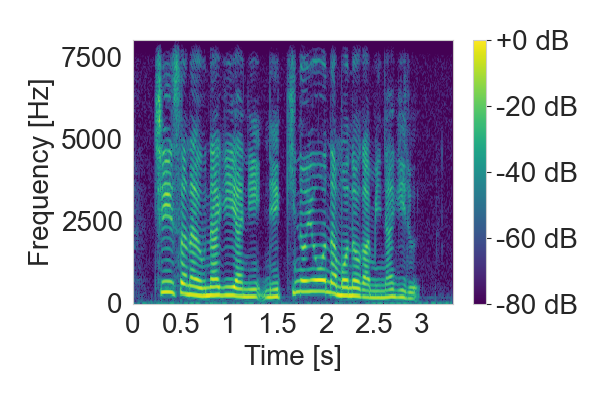
\includegraphics[width=\textwidth]{./figure/sec2/spectrogram_2.png}
        \caption{窓長\SI{25}{\ms},シフト幅\SI{10}{\ms}}
        \label{sec2:fig:spectrogram2}
    \end{subfigure}

    \vspace{0.5cm}

    \begin{subfigure}[b]{0.48\textwidth}
        \centering
        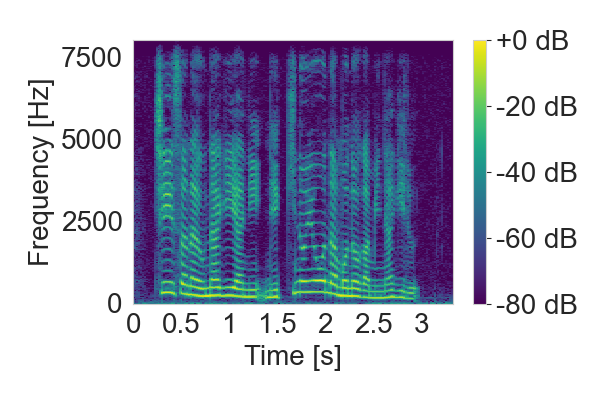
\includegraphics[width=\textwidth]{./figure/sec2/spectrogram_4.png}
        \caption{窓長\SI{50}{\ms},シフト幅\SI{20}{\ms}}
        \label{sec2:fig:spectrogram3}
    \end{subfigure}
    \begin{subfigure}[b]{0.48\textwidth}
        \centering
        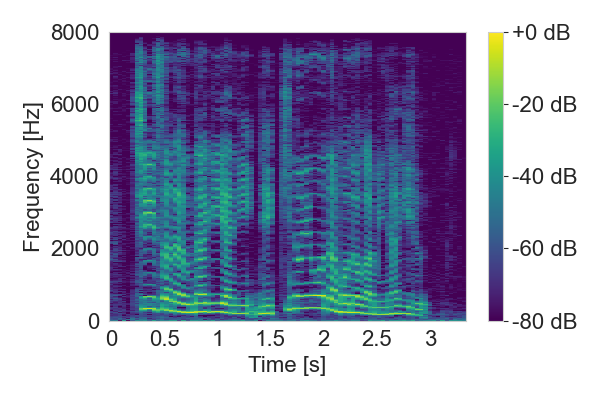
\includegraphics[width=\textwidth]{./figure/sec2/spectrogram_8.png}
        \caption{窓長\SI{100}{\ms},シフト幅\SI{40}{\ms}}
        \label{sec2:fig:spectrogram4}
    \end{subfigure}
    \caption{「小さな鰻屋に,熱気のようなものがみなぎる」と発話した音声から計算された対数パワースペクトログラム}
    \label{sec2:fig:log_power_spectrograms}
\end{figure}

\subsection{メルスペクトログラム}
メルスペクトログラムは,パワースペクトログラムにメルフィルタバンクをかけることによって得られる音響特徴量であり,音声認識や音声合成といったタスクにおいて広く用いられている.パワースペクトログラムを$\bm{X} \in [0, \infty)^{\numUpper_{\text{bin}} \times \timeUpper}$,メルフィルタバンクを$\bm{B} \in [0, 1]^{\numUpper_{\text{mel}} \times \numUpper_{\text{bin}}}$とすると,メルスペクトログラム$\bm{S} \in [0, \infty)^{\numUpper_{\text{mel}} \times \timeUpper}$は
\begin{equation}
    \bm{S} = \bm{B} \bm{X}
\end{equation}
で与えられる.ここで,$\numUpper_{\text{bin}}$は周波数ビンの数,$\numUpper_{\text{mel}}$はフィルタの数,$\timeUpper$はフレーム数である.メルフィルタバンクは,周波数軸を人間の聴感特性を考慮して変換したメル尺度上で,指定した数のフィルタを等間隔に配置して得られる.図\ref{sec2:fig:melfb}に,サンプリング周波数を\SI{16}{\kHz}とした場合におけるメルフィルタバンクを示す.中心周波数の低いフィルタほど帯域幅が狭くなっており,低域ほど細かく,高域ほど荒く周波数成分を扱っていることがわかる.また,フィルタ数を20から80に増やすことによって各フィルタの帯域幅が狭くなり,より細かく周波数成分を考慮できることがわかる.

「小さな鰻屋に,熱気のようなものがみなぎる」と発話した音声に対し,窓長\SI{25}{\ms}のハニング窓を用いてシフト幅\SI{10}{\ms}でパワースペクトログラムを計算し,フィルタ数80のメルフィルタバンクを適用して得られた対数メルスペクトログラムを,図~\ref{sec2:fig:melspectrogram}に示す.

\begin{figure}[tb]
    \centering
    \begin{subfigure}[b]{1.0\textwidth}
        \centering
        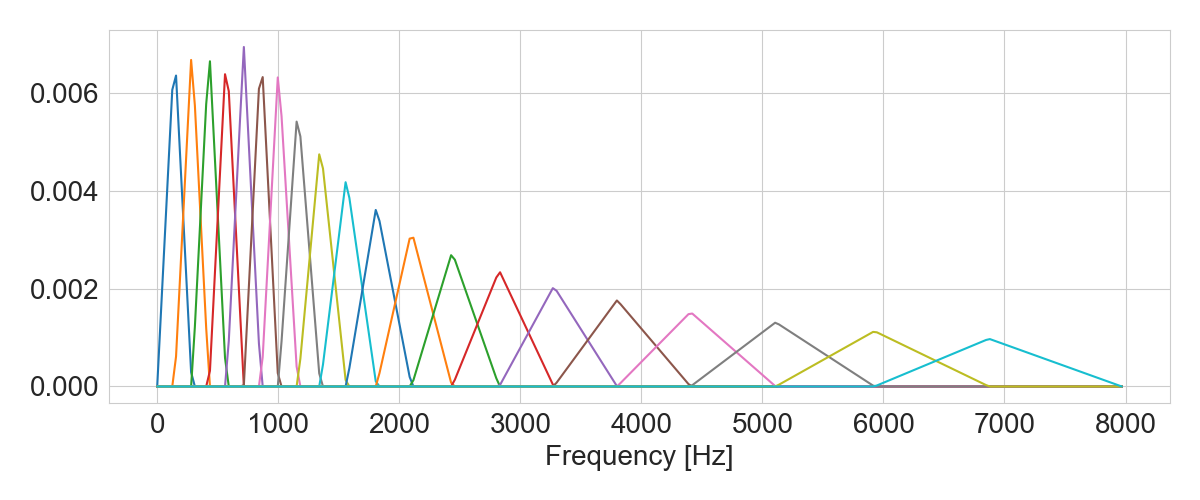
\includegraphics[width=150mm]{./figure/sec2/melfb/onedim_20.png}
        \caption{フィルタ数を20とした場合}
        \label{sec2:fig:melfb_20}
    \end{subfigure}

    \vspace{0.5cm}

    \begin{subfigure}[b]{1.0\textwidth}
        \centering
        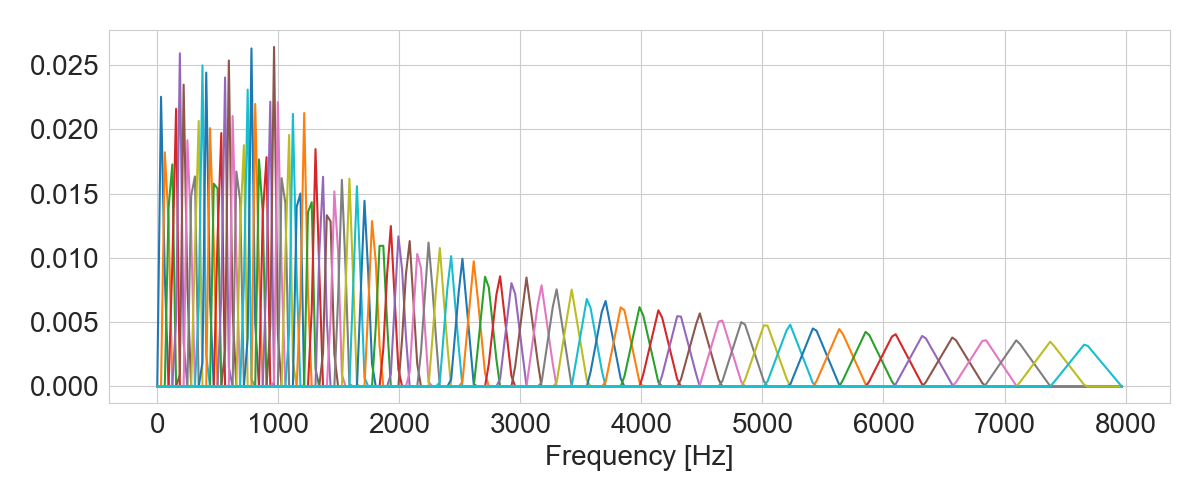
\includegraphics[width=150mm]{./figure/sec2/melfb/onedim_80.png}
        \caption{フィルタ数を80とした場合}
        \label{sec2:fig:melfb_80}
    \end{subfigure}
    \caption{サンプリング周波数を\SI{16}{\kHz}とした場合におけるメルフィルタバンク}
    \label{sec2:fig:melfb}
\end{figure}

\begin{figure}[bt]
    \centering
    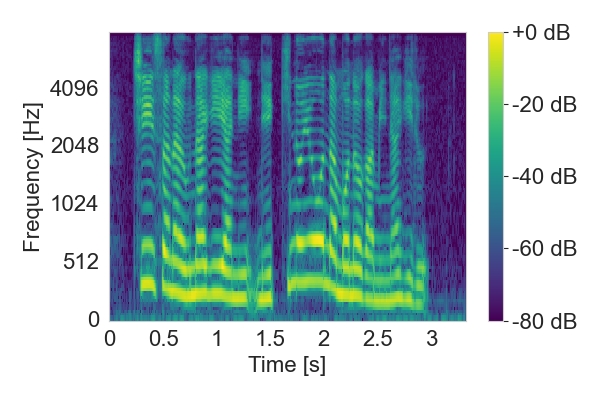
\includegraphics[height=60mm]{./figure/sec2/melspectrogram.png}
    \caption{「小さな鰻屋に,熱気のようなものがみなぎる」と発話した音声に対する対数メルスペクトログラム}
    \label{sec2:fig:melspectrogram}
\end{figure}